\begin{frame}
    \frametitle{Задача поиска выполняющего набора}

    \pause
    \begin{task}
        По булевой формуле $\varphi(x_1, x_2 \dots, x_n)$ найти
        набор $c_1, c_2, \dots, c_n$ такой, что $\varphi(c_1, c_2
        \dots, c_n) = 1$.
    \end{task}

    \pause
    \begin{itemize}
        \item Задача поиска выполняющего набора $NP$-полная.
		\pause
    	\item Множество промышленных задач сводится к задачи поиска
		    выполняющего набора.
        \pause
        \item SAT competition.
    \end{itemize}
\end{frame}

\begin{frame}
    \frametitle{Классы формул}

    \pause
    Для многие классов булевых формул известны эффективные алгоритмы
    для нахождения выполняющего набора:
    \begin{itemize}
        \pause
 		\item $2$-КНФ формулы;
    	\pause
    	\item хорновские формулы;
	    \pause
    	\item цейтинские формулы;
    	\item ...
    \end{itemize}

    \pause
   	Будем рассматривать $d$-КНФ формулы~--- в каждом дизъюнкте не
    более $d$ переменных.
    
    \pause
    $(x_1 \vee x_3 \vee \neg x_5) \wedge (x_2 \vee \neg x_3) \wedge
    (\neg x_2 \vee x_4 \vee x_5) \wedge (x_1 \vee \neg x_4 \vee x_6)$
\end{frame}

\begin{frame}
	\frametitle{Эвристические DPLL алгоритмы}

   	\onslide<1->{
   	\tikzstyle{vertex2} = [opacity = 0]
   	\tikzstyle{vertex3} = [opacity = 0]
    \tikzstyle{vertex4} = [opacity = 0]
   	\tikzstyle{vertex5} = [opacity = 0]
    \tikzstyle{vertex9} = [opacity = 0]
    \tikzstyle{vertex11} = [opacity = 0]
}
\only<2->{\tikzstyle{vertex2} = [opacity = 1]}
\only<3->{\tikzstyle{vertex3} = [opacity = 1]}
\only<4->{\tikzstyle{vertex4} = [opacity = 1]}
\only<5->{
  	\tikzstyle{vertex5} = [opacity = 1]
    \tikzstyle{vertex9} = [opacity = 1]
}

\tikzstyle{end} = [circle, minimum size = 0.6cm, draw, inner sep = 0.1pt]
            
\tikzstyle{level 1} = [level distance = 1.5cm, sibling distance = 5cm]
\tikzstyle{level 2} = [sibling distance = 2cm]
    
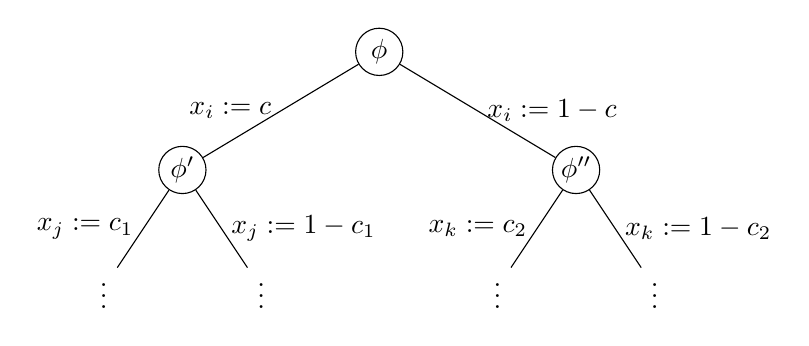
\begin{tikzpicture}[label distance = 8mm]
	\node [end] (z){$\phi$}
       	child [vertex2] {node [end] (b) {$\phi'$}
			child [vertex3]{
	           	node {$\vdots$}
                edge from parent
	  	        node[left] {$x_{j} := c_1$}
            }
		    child [vertex4]{
               	node {$\vdots$}
                edge from parent
	   	        node[right] {$x_{j} := 1 - c_1$}
            }
           	edge from parent
            node[left] {$x_{i} := c$}
        }
        child [vertex5] {node [end] (c) {$\phi''$}
           	child [vertex9]{
               	node {$\vdots$}
                edge from parent
	            node[left] {$x_{k} := c_2$}
            }
		    child [vertex9]{
               	node {$\vdots$}
                edge from parent
	            node[right] {$x_{k} := 1 - c_2$}
            }
            edge from parent
	   	    node[right] {$x_{i} := 1 - c$}
        };
\end{tikzpicture}

    
	\pause
    \pause
    \pause
    \pause
    \pause
    \begin{itemize}
        \item Эвристика $\mathbf{A}$ выбирает переменную.
    	\pause
	    \item Эвристика $\mathbf{B}$ выбирает первое значение.
    \end{itemize}

    \pause
    Разрешим алгоритму ошибаться.

    \pause
    \pause
    \begin{itemize}
	    \item Эвристика $\mathbf{C}$ обрезает ветви.
    \end{itemize}
\end{frame}

\begin{frame}
	\frametitle{Близорукие эвристики}
    \pause
    
    \begin{definition}
        Близорукая эвристика:
        \pause
        \begin{itemize}
	        \item видит структуру формулы;
        	\pause
        	\item не видит знаков отрицаний;
        	\item<6-> на каждом шаге может запросить знаки отрицания в
        		$K = n^{o(n)}$ дизъюнктах.
        \end{itemize}
    \end{definition}

    \pause
    $\begin{array}{l}
        (x_1 \vee x_3 \vee x_5) \\
        \alert<7->{(x_2 \vee x_3)} \\
        (x_2 \vee x_4 \vee x_5) \\
        \alert<7->{(x_1 \vee x_4 \vee x_6)} \\
    \end{array}
    \pause
    \pause
    \pause
    \Rightarrow
    \begin{array}{l}
        (x_1 \vee x_3 \vee x_5) \\
        (x_2 \vee \alert{\neg} x_3) \\
        (x_2 \vee x_4 \vee x_5) \\
        (x_1 \vee \alert{\neg} x_4 \vee x_6) \\
    \end{array}$
    
\end{frame}

\begin{frame}
    \frametitle{Близорукие алгоритмы}

    \pause

    \begin{definition}
		Близорукие алгоритмы:
        \begin{itemize}
            \pause
	        \item $\mathbf{A}$~--- детерминированная, полиномиальная.
            \pause
        	\item $\mathbf{B}$~--- произвольная.
        	\pause
        	\item $\mathbf{C}$~--- близорукая.
        \end{itemize}
	\end{definition}

    \pause
    Если $\mathbf{C} = 1$, то известны некоторые оценки: 

    \pause
    \begin{columns}
        \begin{column}{5cm}
            
            полиномиальное время (верхняя оценка):
        \end{column}
        \begin{column}{5cm}
            
            экспоненциальное время (нижняя оценка):
        \end{column}
    \end{columns}

    \pause
    \begin{columns}
        \begin{column}{5cm}
            \begin{itemize}
		 		\item $2$-КНФ формулы;
			    \pause
    			\item цейтинские формулы (у которых есть выполняющий
			        набор).
            \end{itemize}
        \end{column}
        \begin{column}{5cm}
            \begin{itemize}
	            \pause
    	        \item различные классы невыполнимых формул;
        		\pause
            	\item формулы, кодирующие линейные системы уравнений.
            \end{itemize}
        \end{column}
    \end{columns}
\end{frame}


\begin{frame}
	\frametitle{Функция Голдрейха}
	$f:\{0, 1\}^n \rightarrow \{0, 1\}^n$

    \pause

    \begin{columns}
    	\begin{column}{5.5cm}
            \tikzstyle{end} = [circle, minimum width = 4pt, fill, inner sep = 1pt,
	opacity = 1]
\tikzstyle{start} = [circle, inner sep = 1pt, opacity = 1]
            
\tikzstyle{level 1} = [level distance = 0.1cm, sibling distance = 0.4cm]
\tikzstyle{level 2} = [level distance = 0.45cm]
\tikzstyle{level 3} = [level distance = 1cm]
\tikzstyle{level 4} = [level distance = 0.4cm]

\begin{tikzpicture}[grow = right]
    \node [start]{}
    	child {
        	node [start] (xn) {$x_{n}$}
            	child [end]{
                	node [end] (xvn){}
                    	child [end]{
                        	node [end] (yvn){}
                            	child [start]{
                                	node [start] (yn){}
                                    edge from parent [opacity = 1]
                                }
                            edge from parent [opacity = 0]
                        }
                    edge from parent [opacity = 1]
                }
            edge from parent [opacity = 0]
        }
    	child foreach \i in {3, 2, 1}{
	    	node [start] {}
            	child [start]{
                	node [start] {.}
                    	child [start]{
                        	node [start] {.}
                            edge from parent [opacity = 0]
                        }
                    edge from parent [opacity = 0]
                }
            edge from parent [opacity = 0]
        }
    	child foreach \i in {3, 2, 1}{
	    	node [start] (x\i) {$x_{\i}$}
            	child [end]{
                	node [end] (xv\i){}
                    	child [end]{
                        	node [end] (yv\i){}
                            	child [start]{
                                	node [start] (y\i){}
                                    edge from parent [opacity = 1]
                                }
                            edge from parent [opacity = 0]
                        }
                    edge from parent [opacity = 1]
                }
            edge from parent [opacity = 0]
        };

    \path [draw = red, opacity = 1](xv2) -- (yv2);
    \path [draw = red, opacity = 1](xv3) -- (yv2);
    \path [draw = red, opacity = 1](xvn) -- (yv2);
    \node at (xvn.south) [below = 0.05cm] {$X$};
    \node at (yvn.south) [below = 0.05cm] {$Y$};
    \node <.(2)-> at (y2.east) [right = 0.1cm] {$x_{2} \oplus x_{3}
	    \oplus \dots \oplus x_{n}$};
\end{tikzpicture}

        \end{column}

        \pause
        \pause
        \begin{column}{5.5cm}
            \begin{itemize}
	            \item $f$~--- линейная;
            	\pause
                \item $\forall y \in Y ~~ deg(y) \le d$
            	\pause
            	\item $d$~--- константа.
            \end{itemize}
        \end{column}
	\end{columns}
    
	\pause
	\begin{remark}
	    По уравнению $f_{G, P}(x) = b$ можно построить булеву формулу
		в КНФ, эквивалентную данной системе и формула будет содержать
        не более $2^dn$ дизъюнктов.
	\end{remark}
\end{frame}

\begin{frame}
    \frametitle{Граф зависимостей}

    Двудольный граф $(X, Y, E)$
    \pause
    \begin{itemize}
	    \item Полный ранг матрицы смежности.
    	\pause
        \item Ограниченная степень всех вершин.
    	\pause
        \item Свойства экспандера.
    \end{itemize}

    \pause

    \begin{columns}
        \begin{column}{5cm}
            \tikzstyle{start} = [circle, inner sep = 0pt, opacity = 1]
\tikzstyle{end} = [circle, minimum width = 4pt, fill, inner sep = 1pt,
	opacity = 1]

\onslide<1->{
	\tikzstyle{endY} = [color = black, circle, minimum width = 4pt,
	    fill, inner sep = 1pt, opacity = 1]
	\tikzstyle{endG} = [color = black, circle, minimum width = 4pt,
	    fill, inner sep = 1pt, opacity = 1]
    \tikzstyle{edge} = [draw = black, opacity = 0]
}
\only<6->{
  	\tikzstyle{endY} = [color = red, circle, minimum width = 4pt,
	    fill, inner sep = 1pt, opacity = 1]
    \tikzstyle{edge} = [draw = black, opacity = 1]
}

\only<7->{
  	\tikzstyle{endG} = [color = green, circle, minimum width = 4pt,
	    fill, inner sep = 1pt, opacity = 1]
}
            
\tikzstyle{level 1} = [level distance = 0.1cm, sibling distance = 0.4cm]
\tikzstyle{level 2} = [level distance = 1.5cm]
\tikzstyle{level 3} = [level distance = 1cm]

\begin{tikzpicture}[grow = right]
    \node [start]{}
    	child foreach \i in {10, 9}{
            node [end] (x\i) {}
               	child [end]{
	             	node [end] (y\i){}
    	            edge from parent [opacity = 0]
        	    }
            edge from parent [opacity = 0]
        }
        child foreach \i in {8, ..., 7}{
            node [end] (x\i) {}
               	child [endY]{
	             	node [endY] (y\i){}
    	            edge from parent [opacity = 0]
        	    }
            edge from parent [opacity = 0]
        }
        child foreach \i in {6, ..., 2}{
            node [endG] (x\i) {}
               	child [end]{
	             	node [end] (y\i){}
    	            edge from parent [opacity = 0]
        	    }
            edge from parent [opacity = 0]
        }
        child {
        	node [end] (x1) {}
           		child [end]{
	          		node [end] (y1){}
	    	        edge from parent [opacity = 0]
                }
    	   	edge from parent [opacity = 0]
        };

	\path [edge](y8) -- (x6);
    \path [edge](y8) -- (x4);
    \path [edge](y8) -- (x2);
    \path [edge](y7) -- (x3);
    \path [edge](y7) -- (x5);
    \path [edge](y7) -- (x6);

    \node at (x10.south) [below = 0.05cm] {$X$};
    \node at (y10.south) [below = 0.05cm] {$Y$};

    \path [opacity = 0](y7) -- (y8) node [start, midway] (mid){};
    \node <.(2)-> at (mid.east) [right = 0.05cm] {$J$};
    \node <.(3)-> at (x4.west) [left = 0.05cm] {$\Gamma(J)$};
\end{tikzpicture}
        \end{column}

        \pause
        \pause
        \pause
        \begin{column}{5cm}
            \begin{itemize}
                \item $\forall y \in Y ~~ deg(y) \le d$
            	\pause
	            \item $\forall J \subset Y, ~
            		|J| < r \Rightarrow \Gamma(J) \ge \frac{3}{4}d|J|$
            \end{itemize}
		\end{column}
    \end{columns}

\end{frame}

